\chapter{Quantum state driving}
\label{chap:typesOfDriving}
The concept of quantum state driving was introduced in the previous chapter. In this chapter the initial state is chosen as eigenstate $\ket{s(\llambda)}$. The driving parameter $\llambda$ is changed along path parametrized by time $t$
\begin{equation}
    \mathcal J\coloneqq\{\llambda(t)|t\in[0,T],\; \llambda\in \mathcal U\} \subset \R^n,\quad \llambda(0)=\llambda,\; \llambda(T)=\tilde\llambda,
    \label{eq:defJ_QSdriving}
\end{equation}
inducing the change in Hamiltonian $\HH(\llambda)$ of dim $N$, and consequently in $\ket{\psi(\llambda)}$, according to the Schr\"odinger equation. This leads to solving the system of $N$ first order differential equations with initial condition $\ket{\psi(\llambda(0))}=\ket{o(0)}$.

It is often needed to achieve as high fidelity as possible during the driving, meaning avoiding the state excitation. If $F=1$, we speak about \emph{unit fidelity driving} or \emph{adiabatic driving} and $\mathcal J$ is called the \emph{unit fidelity protocol}. Higher fidelity can be achieved by many methods; three of them are
\begin{itemize}
    \item close adiabatic driving — changing the driving parameters $\llambda$ slowly, so the system has plenty of time to collapse into the ground state,
    \item path variation — varying the driving trajectory $\mathcal J$, avoiding the topological defects on manifolds, which would excite the system,
    \item counter-diabatic driving — countering the excitation by adding some element to the Hamiltonian, making the fidelity precisely $1$.\footnote{There is a nice analogy with driving a toy car \gray{(a quantum state)} in a curved terrain \gray{(a Hilbert space)}. To avoid the car jumping on the hills \gray{(the state excitation)}, you can either drive slowly \gray{(close adiabatic driving)}, or you can go around the hills \gray{(vary the path)}, or you can alter the space for a specific driving \gray{(add a counter-diabatic element)}, such that it exactly copies the jumping trajectory, therefore the car does not leave the ground.}
\end{itemize}

Before going through individual methods, let's look at the adiabaticity itself.

\begin{definition}[Adibaticity]
    The slow change of the driving parameters of the Hamiltonian $H(\llambda)$ in a sense that it does not excite the system and allows the system to return to the same energetic state after circulation around any closed path on the ground state manifold with fidelity $F=1$. 
\end{definition}
This means that adiabatic transport is an endomorphism of $\M _s$. The meaning of the word "slow" clears up the next theorem. It defines when the distance between two states can be considered zero.
\begin{thm}[Adiabatic theorem]
    \label{adiabaticTheorem}
    For slowly varying Hamiltonian $\HH$ in the time range $[0,T]$, the solution of the Schrödinger equation 
    $$\HH(\lambda)\ket{\psi_s(\lambda)} = E_s(\lambda)\ket{\psi_s(\lambda)}$$
    with initial condition in x-representation $\braket{x|\psi(t=0}=\psi(x,0)$ can be approximated as
    \begin{equation}
      ||\psi(\lambda) - \psi_{ad}(\lambda)||\approx o\left(\frac{1}{T}\right)
    \end{equation}
    for the adiabatic state evolved according to Eq. \ref{eq:phasesOnManifold}
    \begin{equation}
        \ket{\psi_{ad}}= e^{\omega_s(\lambda)}e^{\gamma_s(\lambda(t))}\ket{\psi(\lambda)},
    \end{equation}
    for dynamical phase
    $$\omega_s(\lambda)\equiv -\int_0^t E_s(\tau)\d \tau$$
    and geometrical phase
        $$\gamma_s(\lambda(t))\equiv \int_0^t i\braket{\psi_s(\tau)|\partial_t\psi_s(\tau)} \d \tau .$$
\end{thm}
\begin{myproof}
    The proof can be found in \citet[Chap. 6]{sakurai}.
\end{myproof}














\section{Counter-diabatic driving}

Assume differentiable and non-singular Hamiltonian $\HH(\llambda)$ with non-degenerate eigenbasis $\{\ket{s,\llambda}\}_{s=0}^{N-1}$ called the \emph{adiabatic basis}. This is generally the family of adiabatically connected eigenstates\footnote{In the case of energy level crossing, the eigenstates are not unified, because transition between them is not adiabatic.} The transition amplitude between states for adiabatic change is
\begin{equation}
    0=\bra{m(\llambda)}\HH\ket{s(\tilde\llambda)} \quad \text{for }s\neq m, \forall \llambda,\forall \tilde \llambda.
\end{equation}
Differentiation by $\partial_t$ yields
\begin{equation}
    \begin{split}
        0&=\bra{\partial_t m(\llambda)}\HH(\tilde \llambda)\ket{s(\tilde\llambda)}+ \bra{m(\llambda)}\overbrace{\partial_t\HH(\tilde \llambda)}^{\approx \partial_t\HH(\llambda)}\ket{s(\tilde\llambda)}+ \bra{m(\llambda)}\HH(\tilde \llambda)\ket{\partial_t s(\tilde \llambda)}\\
        &=E_s(\llambda)\braket{\partial_t m(\llambda)|s(\tilde \llambda)} + E_m(\llambda)\braket{m(\llambda)|\partial_t s(\tilde \llambda)}+ \bra{m(\llambda)}\partial_t \HH(\tilde\llambda)\ket{s(\tilde \llambda)}\\
        &= (E_m(\llambda)-E_s(\llambda))\underbrace{\braket{m|\partial_t s(\tilde \llambda)}}_{-\frac{i}{\hbar}\bra{m}\AA_t\ket{s(\tilde \llambda)}} + \braket{m|\partial_t\HH|s(\tilde \llambda)},
    \end{split}
\end{equation}
which can be rewritten in matrix form as
\begin{equation}
    i\hbar\partial_t\HH=[\AA_t,\HH]-i\hbar \hat{M}_t\qquad \text{for } \hat{M}_t\equiv -\sum_s\pder{E_s(\lambda)}{t}\ket{s(\lambda)}\!\!\bra{s(\lambda)}.
\end{equation}
$\hat{M}$ is diagonal in energy basis and its elements has meaning of \emph{generalized force}. We can see that $[\HH,\hat{M}]=0$, implying
\begin{equation}
    [\HH,i\hbar\partial_t\HH-[\AA_t,\HH]]=0.
    \label{eq:komutation}
\end{equation}
This equation is essentially the system with constraint $\AA_t$. Its strength lies in the fact that it finds the counter-diabatic potential without Hamiltonian diagonalization. For more, see \citet[Chap. 2.3]{kolodrubez}.










% \subsection{The Hamiltonian gauge transformation}
In section \ref{sec:derivationOfGeometricTensor} we introduced the gauge potential and stated its correspondence to transition probability, see Eq. \ref{eq:probabilityOfTransitionIsGauge}.
\emph{Gauge transformations}, in classical mechanics called \emph{canonical}, can be defined such that they \emph{preserve Lagrangian of the system under local transformations from some Lie group}. The implication is that Hamiltonian $\HH(\llambda)$ commutes with its canonically transformed version.

To understand the meaning of gauge symmetries, let's first consider classical systems and then move to quantum mechanics.




\subsection{Classical gauge potential}
This part is inspired by \citet[Chap. 2.1]{kolodrubez}. In the Hamiltonian classical mechanics, the manifold $\M$ is assumed to be a subset of the phase space defined by Hamiltonian $H=H(q^i,p_i)$, where momentum $p_i$ and position $q^i$ are assumed to form the orthogonal basis of the phase space
\begin{equation}
    \{q^i,p_j\}=\delta^i_j,
    \label{eq:canonicalCommutationDelta}
\end{equation}
which also defines \emph{calibrational freedom} in their choice. \emph{Canonical transformations} then by definition preserve this formula. Using the \emph{Poisson bracket}, defined on observables as
\begin{equation}
    \{A,B\}\coloneqq \pder{A}{q^j}\pder{B}{p_j}-\pder{B}{q^j}\pder{A}{p_j},
\end{equation}
we examine continuous canonical transformations generated by gauge potential $\A_\lambda$
\begin{align}
        q^j(\lambda+\delta\lambda)&=q^j(\lambda)-\pder{\A_\lambda(\bm{p},\bm{q})}{p_j}\delta\lambda \;\Rightarrow\; \pder{q^j}{\lambda}=-\pder{\A_\lambda}{p_j}=\{\A_\lambda,q^j\}
        \label{eq:gaugeAsGeneratorOfMotion1}\\
        p_j(\lambda+\delta\lambda)&=p_j(\lambda)-\pder{\A_\lambda(\bm{p},\bm{q})}{q^j}\delta\lambda \;\Rightarrow\; \pder{p_j}{\lambda}=-\pder{\A_\lambda}{q^j}=\{\A_\lambda,p_j\}.
        \label{eq:gaugeAsGeneratorOfMotion2}
\end{align}
Substituting this to relations of orthogonality \ref{eq:canonicalCommutationDelta}, we get
\begin{equation}
    \{q^j(\lambda+\delta\lambda),p_j(\lambda+\delta\lambda)\}=\delta^i_j + \mathcal{O}(\delta\lambda^2).
\end{equation}
 
If $\lambda$ is time parameter and $\A_t=-H$, equations \ref{eq:gaugeAsGeneratorOfMotion1},\ref{eq:gaugeAsGeneratorOfMotion2} are identical to the Hamilton equations
\begin{equation}
\begin{split}
    \dot{q}^j&=\{q^j,H\} = \pder{H}{p_j}\\
    \dot{p}_j&=\{p_j,H\} = -\pder{H}{q^j}.
\end{split}
\end{equation}
Because the Hamiltonian is a generator of the movement in the phase space $(\bm{q},\bm{p})$, we can interpret $\A_t$ as the generators of the movement on $\M$. Another specific choice might be $\lambda=q^i$, which gives us the momentum components $\A_{q^i}=p_i$.



\subsection{Quantum gauge potential}
This part is inspired by \citet[Chap. 2.2]{kolodrubez}.
Now the aim is to find some special basis transformations $\U$ between the initial system $S$ and the transformed $\tilde{S}$. Both of them describe the system with Hamiltonian $\HH(\llambda)$ with eigenstates $\ket{s(\llambda)}$ on state manifolds $\P\M_s$. 

Any state of $\H(\llambda)$ for $\forall \llambda\in \mathcal U$ can be decomposed as
    \begin{equation}
    \ket{\psi(\llambda)}\equiv \sum_s \psi_s(\llambda)\ket{s}
\end{equation}    
for some coordinate independent basis $\{\ket{s}\}_{s=0}^{N-1}$.
Then there exist unitary transformation
\begin{equation}
    \U(\llambda): \tilde S\rightarrow S,\quad \U(\llambda)\ket{m(\llambda)}=\ket{s}.
    \label{eq:transformationU}
\end{equation}
where scalar parameter $\llambda(t)$ is assumed to be changing along the path $\mathcal J$, therefore we can write the Hamiltonian and states only as functions of $t$. The unitary transformation then satisfies
\begin{equation}
    i\hbar \partial_t \U(t)=\HH(t)\U(t)
    \label{eq:schrodingerForU}
\end{equation}
for $\HH$ the full Hamiltonian of the system and any point on $\mathcal J$, along which the partial derivative is taken.


% The wavefunction $\kpsi$ in $S$ can be decomposed using Schmidt decomposition\footnote{The Schmidt decomposition can be performed in finite dimension, or if the Hamiltonian is compact, which is not automatic in quantum mechanics. What's more, the Hamiltonian is usually not even bounded. Anyway, for simple systems with bounded energy we can assume so.}
% \begin{equation}
%     \ket{\psi(\llambda)} = \sum_{m,s}\psi_n(\llambda) \ket{m(\llambda)}\overbrace{\braket{m(\llambda)|s}}^{U_{ms}(\llambda)} =\sum_m \overbrace{\tilde{\psi}_m(\llambda)}^{\braket{m(\llambda)|\psi_n|s}}\ket{m(\llambda)},
% \end{equation}
% where $U_{ms}(\llambda)$ are matrix elements of unitary transformation $\U(\llambda)$. In this work, we will be interested only in the gauge transformations preserving energy of the system.





% \subsubsection{Adiabatic gauge potential}
The generators of unitary transformations are the adiabatic potentials, which can be defined on wavefunction $\ket{\tilde\psi(\llambda)}$ defined in system $\tilde S$, as
\begin{equation}
    i\hbar\partial_\lambda \ket{\tilde{\psi}(\llambda)} = i\hbar \partial_\lambda\left(\U^+(\llambda)\ket{\psi} \right)= \underbrace{i\hbar\left(\partial_\lambda \U^+(\llambda)\right)\U(\llambda)}_{-\tilde{\AA_\lambda}}\ket{\tilde{\psi}(\llambda)}.
\end{equation}
The adiabatic potential $\tilde{\AA_\lambda}$ can be transformed to non-tilde system as
\begin{equation}
    \begin{split}
        \AA_\lambda&=\U(\llambda)\tilde{\AA_\lambda}\U^+(\llambda) = -i\hbar\U(\llambda)\big(\partial_\lambda \U^+(\llambda)\big) =\\
        &= -i\hbar\partial_\lambda\big(\underbrace{\U^+(\llambda)\U(\llambda)}_{\mathds{1}}\big)-\big(\partial_\lambda \U(\llambda)\big)\U^+(\llambda) \big) =i\hbar \big(\partial_\lambda \U(\llambda)\big)\U^+(\llambda).
    \end{split}
\end{equation}
Now we have explicit formulas for adiabatic potential in two systems
\begin{align}
    \AA_\lambda&=i\hbar \big(\partial_\lambda \U(\llambda)\big)\U^+(\llambda)
    \label{eq:adiabaticPotential}\\
    \tilde{\AA_\lambda} &= -i\hbar\left(\partial_\lambda \U^+(\llambda)\right)\U(\llambda).
    \label{eq:adiabaticPotentialTilde}
\end{align}

The adiabatic potentials can be shown to be Hermitian
\begin{equation}
     \tilde{\AA_\lambda}^+=i\hbar U(\llambda)^+\big(\partial_\lambda\U(\llambda)\big)=-i\hbar\big(\partial_\lambda\U(\llambda)^+\big)\U(\llambda) = \tilde{\AA_\lambda},
     \label{eq:counterdiabaticPotentialTwoSystems}
\end{equation}
analogically for non-tilde potential.

Using the eigenbasis of $\HH$, the matrix elements are
\begin{equation}
    \bra{s}\tilde{\AA_\lambda}\ket{m}=i\hbar\bra{s}\U(\llambda)^+\partial_\lambda\U(\llambda)\ket{m} = i\hbar\bra{s(\llambda)}\partial_\lambda\ket{m(\llambda)}.
\end{equation}
Because
\begin{equation}
    \bra{s(\llambda)}\AA_\lambda\ket{ m(\llambda)}= \bra{s}\tilde{\AA_\lambda}\ket{m},
\end{equation}
we get
\begin{equation}
    \AA_\lambda = i\hbar\partial_\lambda.
    \label{eq:adiabaticPotentialDefinition}
\end{equation}

% It's good to point out that we were applying tilde operators to non-tilde states et vice versa. This can be justified if we consider $\M$ big enough to contain all necessary states, which can be achieved during the transformation.

To see that the gauge potential performs transformation to non-exciting system, one can recall the general form of the adiabatic potential
\begin{equation}
    \bm{\mathcal A}=\big(\bm\nabla U(t)\big)U^{-1}(t) + U(t) \bm{\mathcal A} U^{-1}(t).
\end{equation}
The fact that second element is missing in Eq. \ref{eq:adiabaticPotentialDefinition} implies the space has zero curvature. The curvature $\partial_j A_k(\llambda)-\partial_k A_j(\llambda)$ equals, according to Eq. \ref{eq:geometricTensor}, $\chi_{jk}$.
This means that adiabatic gauge transformations are a class of gauge transformations with $g_{jk}=\Re\chi_{jk}=0$ and according to Eq. \ref{eq:distanceOnM0}, fidelity $F=1$. Therefore, the system is driven by Hamiltonian $\HH(\llambda)$ with fidelity $F<1$, there exists such adiabatic potential $\A_\lambda$, that driving of the same system using $\HH-\A_\lambda$ has unit fidelity.

The adiabatic gauge potentials can then be understood as affine connections defining the parallel transport on fiber bundle, if we define covariant derivative as
\begin{equation}
    D_j\coloneqq\partial_j+i\AA_j,
\end{equation}
which yields $D_j\ket{\psi_n}=0$ for every eigenstate, meaning the transport of eigenvalues on $\P\M_0$ is parallel. $\AA_j$ is generally defined by Eq. \ref{eq:adiabaticPotential}, which gives non-zero covariant derivative for states not belonging to $\P\M_0$. 







% \subsection{Performing counter-diabatic driving}
% This example is taken from \citet{kolodrubez}[page 15--17]. The idea of counter-diabatic driving is that any excitation of the system can be countered by adding the counter-diabatic potential to the Hamiltonian. Consider again any eigenstate $\ket{\psi(\llambda)}$ of the Hamiltonian $\HH=\HH(\llambda)$ driven along the curve $\mathcal J(\llambda(t))$ on $\P\M_0$ depending on time $t$. Because the system is not measured during the driving, it cannot be stated if or if not it was excited, but the main goal here is to achieve fidelity $F=1$, which is iff $\tilde H$ is diagonal along the driving path. For a diagonalizable Hamiltonian, there exists a transformation; see Eq. \ref{eq:transformationU}, for which the fidelity will be zero. Such transformation does not have to be unique, but we can choose any one of them. It can be seen more clearly from a direct transformation of the Schr\"odinger equation. 

% From now on assume $\llambda=\llambda(t)$. The Schrödinger equation
% \begin{equation}
%     i\hbar \der{}{t}\ket{\psi(\llambda)} = \HH(\llambda)\ket{\psi(\llambda)}
% \end{equation}
% can be transformed using 
% \begin{equation}
%     \U(\llambda)^+  \ket{\psi(\llambda)} = \ket{\tilde\psi(\tilde\llambda)},
%     \label{eq:transformationUtimeDependentH}
% \end{equation}
% for which $\tilde H \coloneqq\U^+\HH\U$ is diagonal, leading to
% \begin{align}
%     i\hbar \der{}{t}(\U(\tilde\llambda)\ket{\tilde \psi(\tilde\llambda)}) &= \HH(\llambda)\U(\tilde\llambda)\ket{\tilde \psi(\tilde\llambda)} \\
%     i\hbar \der{\llambda}{t}\partial_\llambda\U(\tilde\llambda)\ket{\tilde \psi(\tilde\llambda)} + i\hbar \U(\tilde\llambda)\der{}{t}\ket{\tilde \psi(\tilde\llambda)} &= \HH(\llambda)\U(\tilde\llambda)\ket{\tilde \psi(\tilde\llambda)}.
% \end{align}

% This can be rewritten using adiabatic potential from Eq. \ref{eq:adiabaticPotentialDefinition}, using \emph{dot} notation for time derivatives and omitting the points in which the objects are evaluated, as
% \begin{equation}
%     i\hbar \der{}{t}\ket{\tilde\psi} = \left[\U^+\HH\U-\dot{\lambda}\tilde{\AA_\lambda}\right]\ket{\tilde\psi} = \left[\tilde H-\dot{\lambda}\tilde{\AA_\lambda}\right]\ket{\tilde{\psi}} \eqqcolon \tilde{H}_m \ket{\tilde{\psi}},
% \end{equation}
% where the term $-\dot{\lambda}\tilde{\AA_\lambda}$ is called \emph{Galilean} and $ \tilde{H}_m$ is the Hamiltonian in transformed system. Because $\tilde{H}$ is diagonal, it drives $\ket{\tilde{\psi}}$ with fidelity $f=1$. This means that for any driving defined by $\HH(\lambda(t))$, which defines the unitary transformation $\U$, there exists such \emph{counter-diabatic potential} $\AA_\lambda$, that $\HH_m + \dot{\lambda}\AA_\lambda$ has $f=1$.


% % Intuition for transformations using original Hamiltonian vs. transformed one can be seen in Fig. \ref{fig:counterdiabaticPotential}. It is good to point out that the eigenstates on this figure belong to the space $\P\M$. However, the paths themselves need to be considered in the whole $\M$, which can be seen as the phase change described by equation \ref{eq:evolutionUduringTransition}.

% % \begin{figure}[h]
% %     \centering
% %     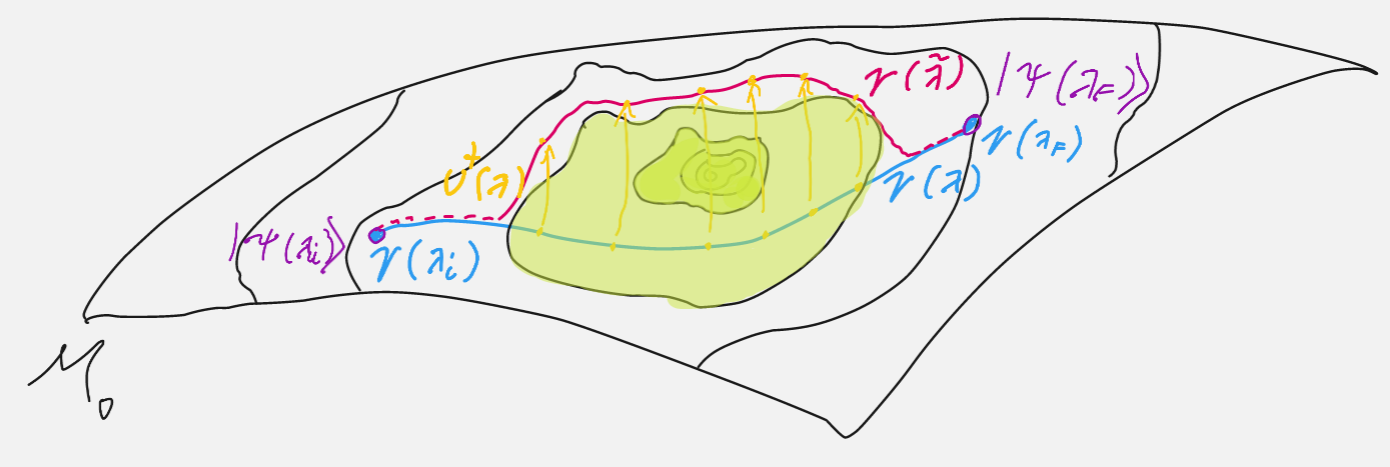
\includegraphics[width=\textwidth]{../img/counterdiabaticPotential.png}
% %     \caption{Comparison between transport by Hamiltonian $\HH$ (blue path $\mathcal J(\lambda)$ and the one with counter-diabatic potential added (pink path $\mathcal J(\tilde\lambda)$), which has zero fidelity. The nonzero fidelity area for path $\mathcal J(\lambda)$ is marked green and initial and final states $\ket{\psi(\lambda_i)}$, resp. $\ket{\psi(\lambda_f)}$ are marked purple.}
% %     \label{fig:counterdiabaticPotential}
% % \end{figure}
% This procedure does not directly tell us how to calculate the counter-diabatic potential, only states its existence. For many simple cases the calculation can be done analytically, but often some approximation methods are needed.


% % \begin{figure}[h]
% %     \centering
% %     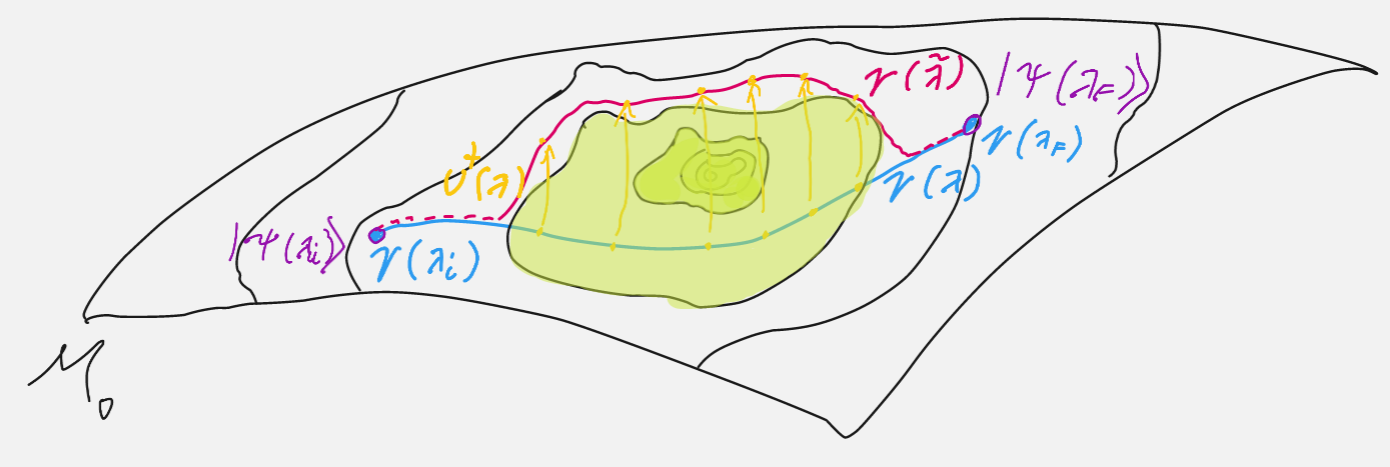
\includegraphics[width=\textwidth]{../img/counterdiabaticPotential.png}
% % \end{figure}




% \subsubsection{Explicit form}
% If we now consider the parametrization with time $t$, $\U$ can be explicitly expressed according to ansatz in Eq. \ref{eq:phasesOnManifold} as
% \begin{equation}
%     \U(t)=\sum_n \exp\left(\frac{i}{\hbar}E_n(\tau)\d \tau - \int_0^t \braket{s(\tau)|\partial_\tau n(\tau)}\d\tau\right)\ket{s(t)}\bra{s(0)}.
%     \label{eq:evolutionUduringTransition}
% \end{equation}
% Inserting to Eq. \ref{eq:schrodingerForU}, we get explicit form of the Hamiltonian, which can be decomposed into the diagonal form of the original Hamiltonian and a counter-diabatic potential
% \begin{equation}
%     \HH(t)=\sum_n \ket{n}E_n\bra{n}+ i\hbar \sum_n\ket{\partial_\lambda n}\bra{n}-\braket{n|\partial_\lambda n}\ket{n}\bra{n}\eqqcolon \HH_0(t)+\HH_1(t),
% \end{equation}
% for shortened notation $\ket{n}\equiv \ket{n(t)}$, analogically for bras. From Eq. \ref{eq:mgradn_proof} we have
% \begin{equation}
%     \HH_0(t)\ket{n}=E_n\ket{n}\quad \Rightarrow\quad \braket{m|\partial_\lambda n}=\frac{\braket{m|\partial_\lambda\HH_0| n}}{E_n-E_m}
% \end{equation}
% and the explicit formula for counter-diabatic element is
% \begin{equation}
%     \HH_1(t)= i\hbar \sum_{m\neq n}\frac{\ket{m}\braket{m|\partial_\lambda\HH_0| n}\bra{n}}{E_n-E_m}
%     \label{eq:explicitCounterDiabaticPotential}
% \end{equation}
























\section{Driving on the ground state manifold}
\label{chap:groundStateManifoldDriving}
As was mentioned in the introduction of chapter \ref{chap:typesOfDriving}, one method of achieving low driving fidelity is \emph{path variation}. It means \emph{finding the best possible driving path}. One might say that the ground state manifold geodesics are a good candidate for this path because they minimize the distance. The problem is that general fidelity driving does not happen on any state manifold, and this premise cannot be used. The natural question here is: "For which drivings do geodesics minimize the fidelity?". The whole role of geodesics is not yet known, but there are a few known cases in which they have particular meaning and which are demonstrated here.

\subsection{Minimizing the distance on state manifolds}
Let's have path $\mathcal J$ with fixed boundary conditions $\llambda(0)=\llambda_i$, $\llambda(T)=\llambda_f$.
The driving on projective ground state manifold $\P\M_0$ then consists of infinitesimal quenches over the distance $\d s$. By integration over this path we get the distance
\begin{equation}
    s_{\mathcal J}=\int\limits_{\mathcal J}\d s=\int\limits_{0}^{T}\sqrt{g_{jk}\dot\llambda^j\dot\llambda^k}\d t
    \label{eq:distancesgamma}
\end{equation}
Let's state and prove the theorem demonstrating the importance of geodesics.
\begin{thm}
    The distance described by formula \ref{eq:distancesgamma} is minimized if $\mathcal J$ is a geodesic.
\end{thm}

\begin{proof}
    Functional of distance is
    \begin{equation}
        s=\int\limits_0^{T} \sqrt{g_{jk}\d\llambda^j\d\llambda^k}=\int\limits_0^{T} \sqrt{g_{jk}\der{\llambda^j}{t}\der{\llambda^k}{t}}\d t \eqqcolon \int\limits_0^{T} \mathcal{L}(t,\llambda^j,\dot\llambda^j)\d t
    \end{equation}
    for 
    \begin{equation}
        \mathcal{L}=\sqrt{g_{jk}\dot\llambda^j\dot\llambda^k}.
    \end{equation}
    Using Euler-Lagrange equations 
    \begin{equation}
        \der{\mathcal{L}}{\llambda^j}-\der{}{t}\der{\mathcal{L}}{\dot\llambda^j}=0,
    \end{equation}
    we get for $g_{jk}=g_{jk}(\llambda)$ second order differential equation
    \begin{equation}
        \ddot\llambda^j+\Gamma^j_{\;\;ab}\dot\llambda^a\dot\llambda^b=0\qquad \Gamma^j_{\;\;ab}=\frac{1}{2}g^{jk}\left(g_{ka,b}+g_{kb,a}-g_{ba,k}\right),
        \label{eq:geodesicEquaiton}
    \end{equation}
    which is the Geodesic equation.
\end{proof}




% \textcolor{blue}{Polkovnikov for some special case: They play a role of "maximum fidelity at any time" transport, meaning at any given time $t$ the fidelity on corresponding point on geodesics will be less than of $\mathcal J$
% $$F(\mathcal{G}(t))<F(\mathcal J(t)).$$ }







\subsection{Minimizing the energy variance}
The driving can be restricted to the ground state manifold only in approximation, such that the excited parts of the wavefunction can be neglected in every step. This fact is used for so-called \emph{close adiabatic drivings}. The first theorem about geodesics is from \citet{Bukov2019}.

\begin{thm}
    \label{thm:polkovnikov}
    For any fast-forward Hamiltonian\footnote{The system is driven to the target state in some fixed final time $T$.} $\HH(\lambda(t))$ driven along one dimensional path $\lambda: \R\mapsto \R$ using time $t$ as parametrization, there exist driving speed, for which the fidelity is close to one, $F(t)\approx 1, \;\forall t\in[0,T]$, and the energy fluctuations $\delta E^2$, averaged along the path, are larger than the geodesic length $l_\lambda$
    \begin{equation}
        \int\limits_0^{T}\sqrt{\delta E^2(t)}\d t \eqqcolon l_t\geq l_\lambda \coloneqq \int\limits_{\lambda_i}^{\lambda_f} \sqrt{g_{\lambda\lambda}\d \lambda\d \lambda} =\int_0^{T} \sqrt{g_{\lambda\lambda}}|\dot \lambda|\d t.
    \end{equation}
    The length $l_\llambda$ is defined in parametric space. For energy variance it holds
    \begin{equation}
        \delta E^2\coloneqq \braket{o(t)|\HH(t)^2|o(t)}-\braket{o(t)|\HH(t)|o(t)}^2=\braket{\partial_t  o(t)|\partial_t o(t)}_c=G_{tt},
    \end{equation}    
    where in second equality the Schr\"odinger equation is used. 
    
    The Metric tensor in parametric space is defined as
    \begin{equation}
        g_{\lambda\lambda}\coloneqq \braket{\partial_\lambda o(t)|\partial_\lambda o(t)}_c,
    \end{equation}
    see Chapter \ref{chap:metricTensor}.
\end{thm}


\begin{proof}
    The essential realization is
    \begin{equation}
        \delta E^2\equiv \braket{o(t)|\HH(t)^2|o(t)}_c=\dot\lambda^2 G_{\lambda\lambda}+\O(\dot\lambda^4),
    \end{equation}
    where $\O(\dot\lambda^4)$ needs to be positive for any real-valued Hamiltonian. The positivity comes from the fact, that the system has instantaneous time-reversal symmetry. For details see \citet{Bukov2019}.
\end{proof}

The conjecture can be extended to an arbitrary dimensional path. The main problem of this conjecture is the statement \emph{close unit fidelity protocol}. It is not clear how good the approximation needs to be. This makes the statement much weaker because it only states that \emph{for any driving, there exists nonzero driving speed for which the energy variance is minimized on geodesics.}









\subsection{Transport using quenches}
\label{sec:quenches}
Unifying the ground states $\ket{o(\llambda)}$ over all points $\llambda\in\mathcal U$ in parametric space, we get the ground state manifold. Here the fidelity $F$ and distance $s$ are
\begin{equation}
    \d s^2 = 1-F(\ket{\llambda+\delta\llambda},\ket{\llambda}) = 1-\left|\braket{o(\bm\llambda+\delta\bm\llambda)|o(\bm\llambda)}\right|^2.
    \label{eq:distanceOnM0_1}
\end{equation}

The final fidelity of transport on $\M$ is then
\begin{equation}
    F=\iint\limits_{\mathcal J} g_{jk}\d\llambda^j\d\llambda^k = \int_{t_i}^{t_f}\underbrace{\int_{t_i}^\tau g_{jk}\der{\llambda^j}{t}\der{\llambda^k}{t} \d t}_{\mathcal{L}(\llambda,\dot\llambda,\tau)}\d \tau .
\end{equation}
From Euler-Lagrange equations, the fidelity is minimized if $\mathcal J$ is geodesic. It is worth mentioning the same problem as was with Theorem \ref{thm:polkovnikov}. It is only stated here that \emph{there exist such slow driving, that the fidelity is minimized on geodesics}. Not how slow this driving needs to be. 
% Using Euler-Lagrange equations for time-independent $g_{jk}=g_{jk}(\llambda)$, leads to
% \begin{equation}
%     \int_{t_i}^{\tau}\left[g_{jk,l}\dot\llambda^j\dot\llambda^k - \der{}{t}\left[g_{jl}\left(\delta^j_k\dot\llambda^k+\dot\llambda^j\delta^k_k\right)\right]\right]\d t=0,
% \end{equation}
% which needs to be zero for integration over any subset $(t_i,\tau)$. This can be achieved for any path only if the integrand itself is zero, which happens if the geodesic equation is satisfied.

% The fidelity $F$ measures transition probability between two eigenstates, $\ket{\psi_1}$, $\ket{\psi_2}$, of different Hamiltonians at two different points $\llambda_1$, $\llambda_2$. These two states belong to the same Fiber space $\PH(\llambda)$ from which the coefficients $$(\text{index of energy state $s$}; \llambda)\in (\Z,\mathcal U)$$ are taken. Because $\PH(\llambda)$ are canonically isomorphic for $\forall \llambda\in \mathcal U$, there is no problem in parallel transport from one space to another, which is needed for evaluating the braket $\braket{\psi(\llambda_1)|\psi(\llambda_2)}$. This is important because the integration in braket can be performed only if both elements belong to the same space.

% The distance minimization runs into some interpretation problems. On the one hand, minimization of the distance is equivalent to maximization of the sum of infinitesimal fidelities along the path (we say we \emph{maximize the fidelity along the path}). On the other hand, we are using only ground states in every step of the transport, therefore defining the fidelity to be one. There are two ways out of this confusion. \emph{Perturbed adiabatic driving} and \emph{transport using quenches}.


Imagine at every point of transport that the fidelity is small enough, so for some small parameter $\delta \llambda\in \R^n$ the transport over distance $\d s$ in eigenbasis at time $t=0$ is
$$\ket{o(\llambda)}\equiv \begin{pmatrix}
    Z_0(\llambda)\\
    0\\
    \vdots \\
    0
\end{pmatrix} \overset{\text{transport }\d s}{\longrightarrow} \ket{o(\llambda+\delta \llambda)}\equiv\begin{pmatrix}
    Z_0(\llambda+\delta \llambda)\\
    0\\
    \vdots \\
    0
\end{pmatrix} +\underbrace{\begin{pmatrix}
    0\\
    \Delta_1(\llambda+\delta \llambda)\\
    \vdots \\
    \Delta_n(\llambda+\delta \llambda)
\end{pmatrix}}_{\mathbf{\Delta}(\llambda+\delta \llambda)}. $$

This has interesting implications for slow transports or small distance transports. For slow transport, the element $\bm\Delta$ increases with time and is hardly fulfilled because one needs to neglect the sum of many of these terms. One possible way out of this is to reset the state into the ground-state when the fidelity would get too far from 1. It can be achieved by projecting the state $\ket{\psi(t)}$ to the ground state $\ket{o(t)}$ periodically. Then because
$$\braket{\Delta(\llambda+\delta\llambda)|o(\llambda+\delta\llambda)}= 0,$$
the fidelity of such driving is almost one. These small jumps are sometimes called \emph{quenches}, and they can be achieved by introducing thermalization to the system.






If we imagine $\delta\llambda$ to be finite (not infinitely small, as the notation suggests), the \emph{transport} means \emph{doing a sequence of quenches and measuring the system after every quench}. This consequently leads to the unit fidelity transport.
% This leads to the \emph{quantum Zeno effect}. In this case it can be shown directly by splitting the distance $s$ on parametric space $\mathcal U$ to $n$ equal pieces. The fidelity for $n$ splits is then
% \begin{equation}
%     F(n)=(1-\Delta s)^n=\left(1-\left(\frac{s}{n}\right)^2\right)^n \;\;\overset{n\rightarrow\infty}{\longrightarrow}\;\; 1,
% \end{equation}
% meaning the consequent measurements on the system leads to collapse to the instantaneous eigenstate and the adiabatic condition for transport holds ($F=1$). 

% Such measurements can be achieved by fast thermalization of the system. If the finite speed thermalization with $N=T/\tau$ for the mean time between two measurements $\tau$, we get
% \begin{equation}
%     \begin{split}
%         \log f(N) &= N \log \left(1-\left(\frac{s}{N}\right)^2\right) = -\frac{s^2}{N}+o\left(\frac{s^4}{n^3}\right)\\
%         f(N) &= \exp\left(-s^2\frac{\tau}{T}-\frac{s^4}{2 N^3}\dots\right) = \exp\left(-s^2\frac{\tau}{T}\right)\left(1+o\left(\frac{s^4}{N^3}\right)\right)
%     \end{split}
% \end{equation}












\section{Adiabatic perturbation theory}
Until now, our interest was mainly in \emph{unit fidelity protocols}. But how to calculate the case when the fidelity is "almost one"? This is the aim of \emph{adiabatic perturbation theory}.


Following the article from \citet{Rigolin2008}, the wavefunction can be approximated by series. Because every element is then decomposed into another series, we bear in mind the \emph{locality of variables}, which clarifies the reason for performing this procedure. Let's call variable $V(\llambda(t))$ \emph{\bluee{local}} if it depends only on the system characteristics in point $\llambda(t)$. These variables can usually be obtained only from the spectrum \bluee{$\sigma(\HH(\llambda(t)))$} and are written in shades of \bluee{blue}. In opposite, a \redd{non-local} variable, written in shades of \redd{red}, depends on the driving path. These are usually expressed as an integral over the driving path $\mathcal J$, but might generally depend on any point which is not on this path.

We are interested in the driving along path $\mathcal J$ defined by Eq. \ref{eq:defJ_QSdriving},
where $t$ is time and $T$ final time of the driving. Let the initial condition be
\begin{equation}
    \ket{\psi(0)}\eqqcolon\ket{\psi_0}\in \P\M_0.
\end{equation}
Solving the Schr\"odinger equation might seem like a straightforward solution. However, if the fidelity is close to 1, the approximate methods are, in comparison with numerical methods, relatively stable. Second reason is, that they might result in an analytical solution to the problem.

The power series is derived using a small parameter $v\coloneqq 1/T$
\begin{equation}
    \red{\ket{\Psi(t)}}=\sum_{p=0}^\infty v^p \red{\ket{\Psi^{(p)}(t)}},
    \label{eq:mainSeries}
\end{equation}
for 
\begin{equation}
    \red{\ket{\Psi^{(p)}(t)}}=\sum_{s=0}^{N-1} e^{-\frac{i}{v} \reddd{\omega_s(t)}}e^{i\reddd{\gamma_s(t)}}\redd{b_s^{(p)}(t)}\bluee{\ket{s(t)}}.
\end{equation}
Here we have
\begin{align}
    \text{dynamical phase }\reddd{\omega_s(t)} &\coloneqq \frac{1}{\hbar}\int_0^t \bluee{E_s(\tau)}\d \tau,\\
    \text{Berry phase }\reddd{\gamma_s(t)} &\coloneqq i\int_0^t \bluee{\braket{s(\tau)|\frac{\d}{\d \tau}s(\tau)}}\d \tau \equiv i\int_0^t \bluee{M_{ss}(\tau)}\d \tau
    \label{eq:gammadef}
\end{align}
and $\bluee{\ket{s(t)}}$ are solutions to
\begin{equation}
    \bluee{\HH(t)\ket{s(t)}}=\bluee{E_s(t) \ket{s(t)}}.
\end{equation}
Variables $\reddd{\omega_s(t)}$ and $\reddd{\gamma_s(t)}$ are defined using integration over the whole protocol, therefore they are \emph{\red{non-local variables}}.
The problem now lies in determining $\redd{b_s^{(p)}(t)}$, which is also \red{non-local}. Because it depends on its relative \reddd{geometrical} and \reddd{dynamical phase} to other \bluee{energy levels}, let's write it as a series
\begin{equation}
    \redd{b_s^{(p)}(t)}=\sum_{m=0}^{N-1} e^{\frac{i}{v}\reddd{\omega_{sm}(t)}}e^{-i\reddd{\gamma_{sm}(t)}}\blue{b_{sm}^{(p)}(t)},
    \label{eq:bnAPT}
\end{equation}
where $\reddd{\omega_{sm}} \coloneqq \reddd{\omega_m}-\reddd{\omega_s}$, $\reddd{\gamma_{sm}} \coloneqq \reddd{\gamma_m}-\reddd{\gamma_s}$.  The reason for \blue{locality} of $\blue{b_{sm}^{(p)}(t)}$ will be clear soon. Inserting all to the original series \ref{eq:mainSeries}, we get
\begin{equation}
    \red{\ket{\Psi(t)}}=\sum_{s,m=0}^{N-1}\sum_{p=0}^\infty v^p e^{-\frac{i}{v}\reddd{\omega_m(t)}}e^{i\reddd{\gamma_m(t)}}\redd{b_{sm}^{(p)}(t)}\bluee{\ket{s(t)}}.
    \label{eq:solve0}
\end{equation}

Because the initial state is an eigenstate of the Hamiltonian at time $t=0$, we get initial condition $\blue{b_{sm}^{(0)}(t)=0}$. In addition, one can rewrite equation \ref{eq:solve0} to the iteratively solvable form
\begin{equation}
    \frac{i}{\hbar}\bluee{\Delta_{sm}(t)}\blue{b_{sm}^{(p+1)}(t)}+\blue{\dot b_{sm}^{(p)}(t)}+\bluee{W_{sm}(t)} \blue{b_{sm}^{(p)}(t)}+\sum_{k=0,k\neq s}\bluee{M_{sk}(t)}\bluee{b_{km}^{(p)}(t)}=0,
    \label{eq:bSolution}
\end{equation}
for $\bluee{\Delta_{sm}(t)}\coloneqq \bluee{E_m-E_s}$, $\bluee{W_{sm}(t)}\coloneqq \bluee{M_{ss}(t)}-\bluee{M_{mm}(t)}$, where $\bluee{M_{ms}}$ is defined in Eq. \ref{eq:gammadef}. We can see that $\blue{b_{ms}^{(p)}}$, as a solution to Eq. \ref{eq:bSolution}, only depends on difference between energy levels, eigenstates during the path and their directional derivatives. Not on the path itself. All of these are easily obtained, once the driving path is prescribed.















% \section{\textcolor{blue}{Approximations of adiabatic potentials}}
% Adiabatic potentials can be calculated from the principal of minimal action, which leads to variational method.

% If the difference between eigenstates of $\HH$ is small, or the generalized force between some states is zero, the computation of the adiabatic potential is numerically unstable. The knowledge of exact adiabatic potential would allow to maintain the system in the ground state thus not exciting it, as the Eigenstate thermalization hypotheses state.

% \begin{hypot}[Eigenstate thermalization hypotheses]
%   For the difference between eigenstates of $\HH$ and extensive thermodynamic entropy $S$, it holds that
%     \begin{equation}
%     E_s-E_m\propto \exp\left(\frac{S}{2}\right).
%   \end{equation}
%   If the states are close, better approximation would be $E_s-E_m\propto \exp(S)$. For matrix elements it holds, that they vanish exponentially with the characteristic scale of the system $a$, i.e.
%   \begin{equation}
%     \bra{m}\AA_\lambda\ket{n} = i\hbar\frac{\braket{m|\partial_\lambda \HH|n}}{E_m-E_s} \propto \exp(-a).
%     \label{eq:thermalizationMatrixElements}
% \end{equation}
% \end{hypot}
% Fortunately in the limit "number of particles" $\rightarrow \infty$ the expression in Eq. \ref{eq:thermalizationMatrixElements} converges.



% \subsection{Variational methods}
% In the case of simple systems, the adiabatic potentials can be found analytically, but for more complicated Hamiltonians we will be forced to use approximations or some perturbational and variational methods.